\chapter{The Graal Compiler Infrastructure} \label{chp:graal}
Graal is a new approach to Java compiler engineering. Here, Graal is introduced and technically assessed. It's strengths and weaknesses are also evaluated.

\section{Background} \label{sec:graal/background}
The basis of the project is the Graal compiler infrastructure \citep{Graal}. Graal is an experimental project developed mainly at Oracle Labs (although there are some additional collaborators at AMD) under the OpenJDK programme.
	
The aim of the Graal project is to develop a Java compiler written in Java itself - `\textit{a quest for the JVM to leverage its own J}'. Graal is, in essence, a Java compiler written in Java. However, this doesn't fully explain the Graal project.
	
Virtually all languages used commonly in industry have had their compilers go through a so-called `bootstrap' process. This bootstrapping process involves writing the compiler for a language in the language it is intended to compile. In many cases the first version of a compiler is written in a different language - commonly used languages include the standard C and C++ due to their performance. There are many examples of this in the real-world - GCC is written in a combination of C and C++\footnote{Although the project is currently converting all C code to C++}, LLVM/Clang is written in C++ etc. There are several advantages to this approach - in essence, this process is a kind of informal proof that the language has matured to a level that is capable of supporting a program as complicated as a compiler. In effect, bootstrapping a compiler displays shows that a language (and associated platform) has a certain level of `maturity', that it is now ready for large software projects (or at least not totally unprepared for one).

Graal is an attempt to bring this approach to the Java language. Note that there are other projects with attempts to bootstrap parts of the Java platform - for example, the Maxine VM is a Java virtual machine written in Java. However, because Java is unlike most other platforms (in that it not only requires a compiler, but also a virtual machine, class library and such), the compiler has, until the advent of the Graal project, remained written in C++.

Another feature of Graal is that it allows users (of the compiler) to interface directly with the compiler. Common compilers (GCC, ICC etc) are seen as `black-boxes', where a user invokes the compiler, waits for a while, and then a resulting object file or binary is produced. Graal is a part of a new generation of compilers that expose APIs to users, which means users can change parts of the compilation process to suit their needs, ease debugging and other such advantages. With modern languages and platforms being required to target multiple different machine classes (module, desktop, laptop and server/cloud), this is a crucial advantage over more conventional languages and platforms. There are only a few examples of this new generation of compiler, but another - somewhat more mainstream example - is Microsoft's Rosyln project for their .NET platform. The new Windows Runtime include deep metadata integration into the platform (which is the basis for, amongst other things, the Common Object System in .NET languages\footnote{Which allows inter-language types to be considered equivalent - a C int is semantically equivalent to a C++ int, a C\# int, a JavaScript int and so on}).

\section{Introduction} \label{sec:graal/introduction}
Graal is somewhat different than other compilers. As opposed to other compilers, which use a combination of parsers and lexers to produce their IRs from source code, Graal builds the IR from Java bytecode instead. This approach has several advantages for this project, the main being that we cannot assume that the source code is available to many legacy programs. Another advantage to this approach is that it would allow the detection mechanism to not only be performed upon user-provided programs, but also system-level libraries as well (for example, the Java Collections Framework). 

\section{Intermediate Representations} \label{sec:graal/ir}
Like many compilers, Graal uses several different internal representations at different stages of compilation. Each of the representations has a distinct, non-overlapping use case; despite this the graphs are somewhat similar in structure.

As is common in many compilers, Graal uses graphs for intermediate representations. These graphs combine several different kinds of graph together into a single form, such as control flow and memory dependency (data flow).

To illustrate this, consider the figure \ref{fig:vector-inline}, created using the Ideal Graph Visualiser (\textit{IGV}).

\begin{figure}
	\centering
	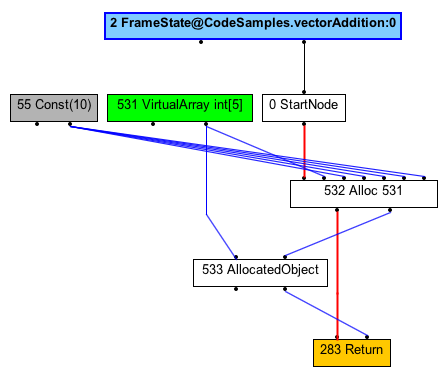
\includegraphics[width=0.7\textwidth]{graphics/loop-inline.png}
	\caption{Graal HIR created for a vector addition using two array literals}
	\label{fig:vector-inline}
\end{figure}

The format for graph visualisations is the following:
\begin{itemize}
	\item Red edges represent control flow
	\item Blue edges represent memory dependence
	\item Black edges are defined as edges which are not control flow or memory dependence. In reality, they are mainly used for associating \texttt{FrameState} nodes where appropriate
\end{itemize}

The text inside nodes uses the following format:

\texttt{<node-id> NodeName <additional>}

In some cases, \texttt{<additional>} contains the value associated with the code (for subtypes of \texttt{ValueNode}). Node IDs are unrelated to the ordering within the graph. Time is represented on the y-axis of the graph, flowing down the page.

\autoref{fig:vector-inline} is a representation of a vector addition using two \texttt{int} array literals as arguments. The original source code contains a loop, which itself contains two array load operations, an addition and an array store operation. From it, we can see clearly the different kinds of node relationships in Graal's IR. The \texttt{StartNode} is the start of the method, which is followed by an allocation (notice that the loop was been optimized away by Graal), the result of which is then returned from the method.

The allocate has two actual memory dependencies:

\begin{itemize}
	\item A \texttt{VirtualArray} node is used to create an array. We can see that the type of this array is \texttt{int[]} with length five.
	
	\item A \texttt{ConstantNode} is referenced five times, one for each position of the array.
\end{itemize}

Without both of these dependencies, the compiler cannot create the array, and assign the correct values. Note that, because the JVM allocates default values of zero to declared-yet-unassigned variables, if the \texttt{ConstantNode} was not used, the array would consist of zeros.

\section{Graph Transformations} \label{sec:graal/transformations}
One of the ways the abilities of Graal are manifested is through it's capacity to apply transformations to the various intermediate representations. The main use for this is to allow users of the compiler to add custom behaviour at the various stages of the compilation process, but the mechanism extends to additional uses. For example, custom behaviour can be inserted into programs, as well as the graphs dumped for inspection in external tools\footnote{One such tool is the `Ideal Graph Visualiser', which is included in the Graal repository.}.

As of the time of writing, Graal uses a hybrid approach to transforming graphs between the IRs - suites and phases. They are, in effect, essentially the same thing - they both consist of a sequence of transformations (in Graal terminology, a \textit{phase}) which are applied to a graph in a well-defined order (although the user can change the ordering if required, as well as disable certain phases via \texttt{com.oracle.graal.phases.PhasePlan.disablePhase()}. The result of a sequence of phases is the representation used at the next lower-level of abstraction. The three phases in Graal are high-level, mid-level, and low-level.

\small{\textit{Todo: clear up the difference between runtime-specific lowering and target-specific lowering.}}

The high-level phase is used mainly for the graph-building phase. Graal uses the concept of \texttt{ResolvedJavaMethod}s, which are internal `linkages' to constant pools found within \texttt{.class} files. It is also used for runtime-specific lowering\footnote{\emph{Lowering} is a mechanism to convert a complex bytecode into a simpler one, much like the difference between RISC and CISC architectures}, for example to handle multiple machine instruction set architectures - although the Java language is unconcerned with JVM implementation details such as the endianness of the machine's CPU, the runtime must, by definition, be aware of this fact. Examples of runtime-specific lowering are found throughout Graal, but examples include multiple implementations of the \texttt{GraalRuntime} interface - one for each ISA that Graal supports. Single Static Assignment (SSA) form is used at the high-level in order to allow for optimisations to be performed.

Mid-level phases remove the SSA form, and includes target-specific lowering. The low-level phases are analogous to the backends of more traditional compilers, and deals with low-level issues such as register allocation and code generation.

	\subsection{The \texttt{.class} File Format - Constant Pools}
	In order to properly understand \texttt{ResolvedJavaMethod}s, one needs to understand some parts of the \texttt{.class} file format. The source for this section is the Java Virtual Machine specification \citep[p.~69]{JVMSpec}.
		
	\texttt{.class} files are structured containers for Java bytecode streams. However, they are not `plain old data structures', as would be indicated by that description. Instead, they are laid out in such a way to increase performance for the JVM.
				
	Unlike some other executable file formats, the JVM does not rely on the (relative) positions of the various kinds of definition permitted. In this context, constants refer to \emph{all} immutable identifiers - and not simply to the language-level construct of constants (\eg, \texttt{public static final int THOMAS\_KLAUS = 9;}). Each constant has an entry in the \emph{constant pool} - a table containing \texttt{cp\_info} structures. A \texttt{ResolvedJavaMethod} contains a link to the offset of a \texttt{cp\_info} structure for a method.